\documentclass[../../../../main.tex]{subfiles}
\begin{document}

\section*{第1問}

\begin{center}
\begin{tikzpicture}[scale=2.5]
    % Coordinates
    \coordinate (O) at (0,0);
    \draw (O) circle (1);
    
    % Radius 1 circle points A1 to A6
    \foreach \i in {1,...,6} {
        \coordinate (A\i) at ({90 - (\i-1)*60}:1);
    }
    
    % Draw radii to A1, A6, A3, A4, A5
    \draw (O) -- (A1) node[above] {$A_1$};
    \draw (O) -- (A6) node[above right] {$A_6$};
    \draw (O) -- (A3) node[below left] {$A_3$};
    \draw (O) -- (A4) node[below] {$A_4$};
    \draw (O) -- (A5) node[below right] {$A_5$};
    \draw (O) -- (A2) node[above left] {$A_2$};

    % Small circle inside angle A1-O-A6
    % Angle is 60 deg, bisector is 60 deg (pi/3) from x-axis, i.e., 60 deg in standard angle (between 90 and 30 deg) -> 60 deg angle relative to origin
    % Radius r = 2\sqrt{3} - 3 \approx 0.4641
    % OP = r / sin(30) = 2r \approx 0.9282 at angle 60 deg
    \coordinate (P) at (60:0.5359); % OP = 1 - r = 1 - 0.4641 = 0.5359
    \draw (P) circle (0.4641);
    \node[above] at (P) {$P$};
    \node right at (P) {$r$};

    % Points C, Q
    \coordinate (C) at (120:0.5359);
    \coordinate (Q) at (240:0.5359);
    \coordinate (B) at (0, 0.2);

    \draw (O) -- (P);
    \draw (O) -- (C);
    \draw (P) -- (C);
    \draw (C) -- (Q);
    \draw (P) -- (Q);

    \node[below left] at (Q) {$Q$};
    \node[left] at (C) {$C$};
    \node[left] at (O) {$O$};
    
    % Shaded region indicator
    \draw[thick, red, opacity=0.5] (A1) arc (90:210:1) -- (Q) -- (P) -- cycle;
\end{tikzpicture}
\end{center}

\noindent
\textbf{[解]}

$P$ を中心とする円の半径を $r$ とすると、$OA_1 = OP + PA_1$ より
\[
1 = r + \frac{r}{\sin \frac{\pi}{3}} = \left( \frac{2}{\sqrt{3}} + 1 \right) r = \left( \frac{2}{3}\sqrt{3} + 1 \right) r
\]
\[
\therefore r = -3 + 2\sqrt{3} \quad \cdots \text{①}
\]

題意から、$QC = OP$, $CP = QO$ だから、$\square OPCQ$ は平行四辺形である。

求める面積を $S$ とすると、図形の和・差に分解して考える：

\begin{center}
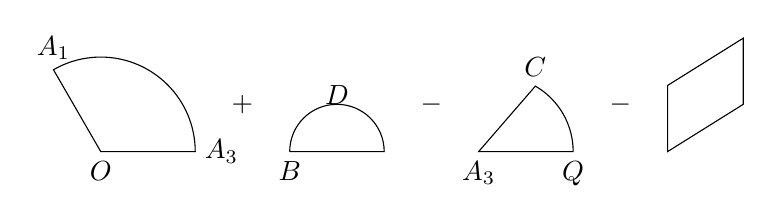
\begin{tikzpicture}[scale=1.2]
    % Diagrams of decomposition
    % Sector OA1A3
    \draw (0,0) node[below]{$O$} -- (1,0) node[right]{$A_3$} arc(0:120:1) node[above]{$A_1$} -- cycle;
    \node at (1.5, 0.5) {$+$};

    % Region D
    \draw (2,0) node[below]{$B$} -- (3,0) arc(0:180:0.5) -- cycle;
    \node at (2.5, 0.6) {$D$};
    \node at (3.5, 0.5) {$-$};

    % Region CQ A3
    \draw (4,0) node[below]{$A_3$} -- (5,0) node[below]{$Q$} arc(0:60:0.8) node[above]{$C$} -- cycle;
    \node at (5.5, 0.5) {$-$};

    % Parallelogram region
    \draw (6,0) -- (6.8, 0.5) -- (6.8, 1.2) -- (6, 0.7) -- cycle;
\end{tikzpicture}
\end{center}

各部分の面積は：
\begin{itemize}
    \item 扇形 $OA_1A_3$: $\frac{1}{2} \cdot \frac{2}{3}\pi = \frac{\pi}{3}$
    \item 半円領域 $D$: $\frac{1}{2}\pi r^2$
    \item 扇形 $Q C A_3$: $\frac{1}{2} \cdot \frac{2}{3}\pi (1-r)^2 = \frac{1}{3}\pi (1-r)^2$
    \item 平行四辺形 $OPCQ$ から扇形を除いた部分:
    \[
    (1-r) \cdot r \cdot \sin \frac{\pi}{3} - \frac{1}{6}\pi r^2 = \frac{\sqrt{3}}{2}(r - r^2) - \frac{1}{6}\pi r^2
    \]
\end{itemize}

だから、代入して
\begin{align*}
S &= \frac{\pi}{3} + \frac{1}{2}\pi r^2 - \frac{1}{3}(1-r)^2\pi - \left\{ \frac{\sqrt{3}}{2}(r-r^2) - \frac{1}{6}\pi r^2 \right\} \\
&= \pi \left\{ \frac{1}{3} + \frac{1}{2}r^2 - \frac{1}{3}(1-r)^2 + \frac{1}{6}r^2 \right\} - \frac{\sqrt{3}}{2}(r-r^2) \\
&= \frac{\pi}{6} \left[ 2r^2 + 4r \right] - \frac{\sqrt{3}}{2} r (1-r)
\end{align*}

ここで、①より $r^2 = (-3+2\sqrt{3})^2 = 21 - 12\sqrt{3}$ だから
\begin{align*}
S &= \frac{\pi}{3} \left\{ (21 - 12\sqrt{3}) + 2(-3 + 2\sqrt{3}) \right\} - \frac{\sqrt{3}}{2} \left\{ (-3 + 2\sqrt{3}) - (21 - 12\sqrt{3}) \right\} \\
&= \frac{\pi}{3} \left[ 15 - 8\sqrt{3} \right] - \frac{\sqrt{3}}{2} \left( -24 + 14\sqrt{3} \right) \\
&= (15 - 8\sqrt{3})\frac{\pi}{3} - 21 + 12\sqrt{3} \\
&= (5\pi - 21) + \left( 12 - \frac{8}{3}\pi \right)\sqrt{3}
\end{align*}

\newpage

\section*{第2問}

\noindent
\textbf{[解]}

\[
f(x) = (x+2)(x-2)(x+3)(x-3) \quad \cdots \text{①}
\]
とおく。
\begin{align*}
f(t+1) = f(t) &\iff (t+3)(t-1)(t+4)(t-2) = (t+2)(t-2)(t+3)(t-3) \\
&\iff (t+3)(t-2) \left[ t^2 + 3t - 4 - (t^2 - t - 6) \right] = 0 \\
&\iff (t+3)(t-2)(4t+2) = 0
\end{align*}
に注意してグラフを描くと以下のようになる。

\begin{center}
\begin{tikzpicture}[scale=0.8]
    \draw[->] (-4,0) -- (4,0) node[right] {$x$};
    \draw[->] (0,-1) -- (0,4.5) node[above] {$y$};
    \draw[domain=-3.2:3.2, smooth, variable=\x, blue, thick] plot ({\x}, {0.05*(\x+2)*(\x-2)*(\x+3)*(\x-3) + 3.6});
    \node[above left] at (0,3.6) {極大 (36)};
    \draw[dashed] (-3,0) node[below]{$-3$} -- (-3,3.6);
    \draw[dashed] (-2,0) node[below]{$-2$} -- (-2,3.6);
    \draw[dashed] (-1,0) node[below]{$-1$} -- (-1,3.6);
    \draw[dashed] (-0.5,0) node[below]{$-\frac{1}{2}$};
    \draw[dashed] (0.5,0) node[below]{$\frac{1}{2}$};
    \draw[dashed] (2,0) node[below]{$2$};
    \draw[dashed] (3,0) node[below]{$3$};
\end{tikzpicture}
\end{center}

従って、
\[
g(t) = \begin{cases}
f(t+1) & (-3 \le t \le -1) \\
36 & (-1 \le t \le 0) \\
f(t) & (0 \le t \le 2) \\
f(t+1) & (2 \le t \le 3)
\end{cases}
\]
だから、図示して下図のようになる。

\begin{center}
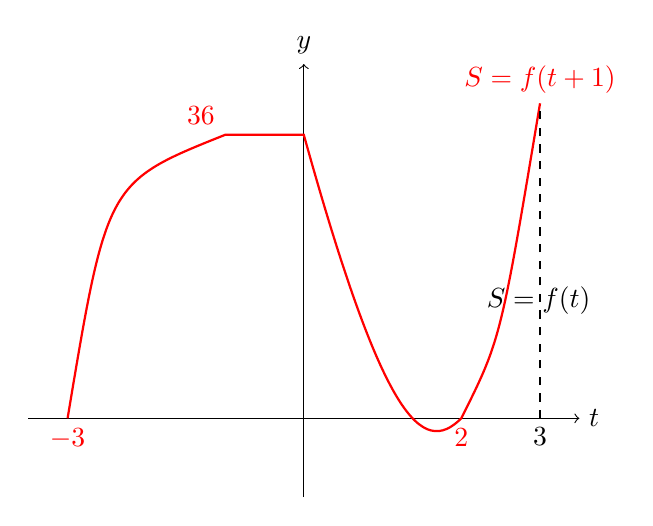
\begin{tikzpicture}[scale=1.0]
    \draw[->] (-3.5,0) -- (3.5,0) node[right] {$t$};
    \draw[->] (0,-1) -- (0,4.5) node[above] {$y$};
    
    % g(t) plot
    \draw[thick, red] (-3,0) node[below]{$-3$} 
        .. controls (-2.5, 3) .. (-1, 3.6) node[above left]{$36$}
        -- (0, 3.6)
        .. controls (1, 0) and (1.5, -0.5) .. (2, 0) node[below]{$2$}
        .. controls (2.5, 1) .. (3, 4) node[above]{$S=f(t+1)$};

    \node[right] at (2.2, 1.5) {$S=f(t)$};
    \draw[dashed] (3,0) node[below]{$3$} -- (3,4);
\end{tikzpicture}
\end{center}

\newpage

\section*{第3問}

\noindent
\textbf{[解]}

$f(x) = \frac{3}{2}x^2 - \frac{1}{3}$ とおく。$f'(x) = 3x$ より、$Q\left(t, f(t)\right)$ における法線は
\[
(x-t) + 3t \left( y - \frac{3}{2}t^2 + \frac{1}{3} \right) = 0 \quad \cdots \text{①}
\]
と書ける。

\medskip
\noindent
(1) $P(X, Y)$ とする。①が $P$ を通るとき
\[
(X-t) + 3t \left( Y - \frac{3}{2}t^2 + \frac{1}{3} \right) = 0 \quad \cdots \text{②}
\]
放物線では接点が異なれば法線も異なるので、②を満たす $t$ がただ1つあるような $X, Y$ の条件を求めれば良い。②を整理して
\[
9t^3 - 6Yt - 2X = 0 \quad \cdots \text{③}
\]
この左辺を $g(t)$ とおく。$g'(t) = 27t^2 - 6Y$ より、$Y$ によって以下の場合に分かれる。

\paragraph{1. $Y \le 0$ の時}
$g'(t) \ge 0$ だから、$g(t)$ は単調増加。これと $g(t)$ が3次関数であることから、③はただ1つの実根を持つ。

\paragraph{2. $Y > 0$ の時}
増減表は以下の通り：
\begin{center}
\begin{tabular}{c|ccccc}
$t$ & $\dots$ & $-\sqrt{\frac{2Y}{9}}$ & $\dots$ & $\sqrt{\frac{2Y}{9}}$ & $\dots$ \\
\hline
$g'$ & $+$ & $0$ & $-$ & $0$ & $+$ \\
\hline
$g$ & $\nearrow$ & 極大 & $\searrow$ & 極小 & $\nearrow$
\end{tabular}
\end{center}

したがって、グラフの概形から条件は
\[
g\left(\sqrt{\frac{2Y}{9}}\right) g\left(-\sqrt{\frac{2Y}{9}}\right) > 0 \quad \cdots \text{④}
\]
である。③から
\[
g\left(\pm \sqrt{\frac{2Y}{9}}\right) = \pm 9 \left(\frac{2Y}{9}\right)^{\frac{3}{2}} \mp 6Y \sqrt{\frac{2Y}{9}} - 2X = \mp \frac{4}{3}Y\sqrt{Y} - 2X \quad (\text{複号同順})
\]
だから、④に代入して
\[
\left( \frac{4}{3}Y\sqrt{Y} - 2X \right) \left( -\frac{4}{3}Y\sqrt{Y} - 2X \right) > 0 \quad \cdots \text{⑤}
\]

以上1. 2. から、求める領域は
\[
Y \le 0 \quad \text{または} \quad \left( Y > 0 \ \text{かつ}\ \left( \frac{2\sqrt{2}}{3}Y^{\frac{3}{2}} - X \right)\left( \frac{2\sqrt{2}}{3}Y^{\frac{3}{2}} + X \right) < 0 \right)
\]
で、図示して下図斜線部（境界を含む）。

\begin{center}
\begin{tikzpicture}[scale=1.2]
    \draw[->] (-2.5,0) -- (2.5,0) node[right] {$x$};
    \draw[->] (0,-1) -- (0,2) node[above] {$y$};
    \draw[domain=0:1.5, smooth, variable=\y, thick] plot ({ (2*sqrt(2)/3)*(\y^1.5) }, {\y});
    \draw[domain=0:1.5, smooth, variable=\y, thick] plot ({ -(2*sqrt(2)/3)*(\y^1.5) }, {\y});
    \node[right] at (1.2, 1.2) {$x = \frac{2\sqrt{2}}{3}y^{\frac{3}{2}}$};
    \node[left] at (-1.2, 1.2) {$x = -\frac{2\sqrt{2}}{3}y^{\frac{3}{2}}$};
    % Hatching inside region Y > 0 and Y <= 0
    \fill[pattern=north east lines, pattern color=gray!60] (-2.5,-1) rectangle (2.5,0);
    \fill[pattern=north east lines, pattern color=gray!60] plot[domain=0:1.5] ({ (2*sqrt(2)/3)*(\y^1.5) }, {\y}) -- plot[domain=1.5:0] ({ -(2*sqrt(2)/3)*(\y^1.5) }, {\y}) -- cycle;
\end{tikzpicture}
\end{center}

\medskip
\noindent
(2) 対称性から、$x \ge 0$ のうちで題意を満たす面積を $S_1$、題意の面積を $S$ として
\[
S = 2 S_1 \quad \cdots \text{⑥}
\]
である。$S_1$ は右図斜線部の面積で、$y = f(x)$ と $x = \frac{2\sqrt{2}}{3}y^{\frac{3}{2}}$ の $x>0$ での交点の $y$ 座標を $y_0$ とすると、$x$ を消去して
\[
y_0 = \frac{3}{2} \cdot \frac{8}{9} y_0^3 - \frac{1}{3} \implies 4y_0^3 - 3y_0 - 1 = 0 \implies (y_0 - 1)(4y_0^2 + 4y_0 + 1) = 0
\]
から、$y_0 > 0$ より $y_0 = 1$。このときの $x$ 座標は $x = \frac{2\sqrt{2}}{3}$ である。

\begin{center}
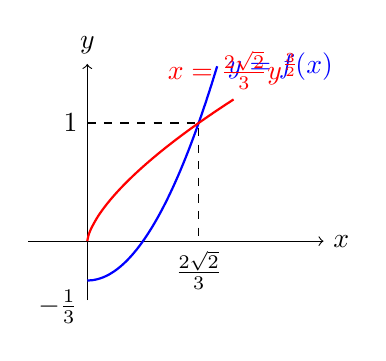
\begin{tikzpicture}[scale=1.5]
    \draw[->] (-0.5,0) -- (2,0) node[right] {$x$};
    \draw[->] (0,-0.5) -- (0,1.5) node[above] {$y$};
    \draw[domain=0:1.1, smooth, variable=\x, blue, thick] plot ({\x}, {1.5*\x*\x - 1/3}) node[right]{$y=f(x)$};
    \draw[domain=0:1.2, smooth, variable=\y, red, thick] plot ({ (2*sqrt(2)/3)*(\y^1.5) }, {\y}) node[above]{$x=\frac{2\sqrt{2}}{3}y^{\frac{3}{2}}$};
    \draw[dashed] (0,1) node[left]{$1$} -- ({2*sqrt(2)/3}, 1) -- ({2*sqrt(2)/3}, 0) node[below]{$\frac{2\sqrt{2}}{3}$};
    \node[below left] at (0,-1/3) {$-\frac{1}{3}$};
\end{tikzpicture}
\end{center}

\[
S_1 = (\text{領域 } D) - (\text{領域 } \Delta) \quad \cdots \text{⑦}
\]
で、
\[
D = \text{矩形} - \int_0^{\frac{2\sqrt{2}}{3}} \left\{ f(x) + \frac{1}{3} \right\} dx = \frac{4}{3} \cdot \frac{2\sqrt{2}}{3} - \frac{1}{2} \left[ x^3 \right]_0^{\frac{2\sqrt{2}}{3}} = \frac{16}{27}\sqrt{2} \quad \cdots \text{⑧}
\]
\[
\Delta = \int_0^1 \frac{2\sqrt{2}}{3} y^{\frac{3}{2}} dy = \frac{2\sqrt{2}}{3} \left[ \frac{2}{5} y^{\frac{5}{2}} \right]_0^1 = \frac{4\sqrt{2}}{15} \quad \cdots \text{⑨}
\]
よって、⑧⑨を⑦に代入して
\[
S_1 = \frac{16}{27}\sqrt{2} - \frac{4}{15}\sqrt{2} = \frac{44}{135}\sqrt{2}
\]
⑥から
\[
S = \frac{88}{135}\sqrt{2}
\]

\newpage

\section*{第4問}

\noindent
\textbf{[解]}

単位行列を $I$ とおく。ケーリー・ハミルトンの定理から、
\[
A^2 - \left(\frac{1}{3} + 3\right) A + \det(A) \cdot I = 0 \implies A^2 = \frac{10}{3}A - I \quad \cdots \text{①}
\]
である。したがって、$n \in \mathbb{N}_{\ge 2}$ に対し、
\[
A^{n+1} = A^{n-1} \cdot A^2 = A^{n-1} \left( \frac{10}{3} A - I \right) = \frac{10}{3} A^n - A^{n-1} \quad \cdots \text{②}
\]
となる。ここで、数列 $c_n$ が $c_{n+2} = \frac{10}{3} c_{n+1} - c_n$ を満たすとき、その一般項は $p, q$ を定数として
\[
c_n = 3^n p + \left(\frac{1}{3}\right)^n q
\]
で与えられることに注意する。

\medskip
\noindent
(1) $A = \begin{pmatrix} 1/3 & 5 \\ 0 & 3 \end{pmatrix}$, $A^2 = \begin{pmatrix} 1/9 & 50/9 \\ 0 & 9 \end{pmatrix}$ である。ここで
\[
A^n = 3^{n-1} \begin{pmatrix} 0 & 45/8 \\ 0 & 3 \end{pmatrix} + \left(\frac{1}{3}\right)^{n-1} \begin{pmatrix} 1/3 & -5/8 \\ 0 & 0 \end{pmatrix} = \begin{pmatrix} (1/3)^n & (3^n - (1/3)^n)\frac{15}{8} \\ 0 & 3^n \end{pmatrix} \quad \cdots \text{③}
\]
であることを帰納的に示す。$n=1,2$ の時は成立する。そこで $n=k, k+1 \ (k \in \mathbb{N})$ での③の成立を仮定すると、②から
\begin{align*}
A^{k+2} &= \frac{10}{3} \begin{pmatrix} (1/3)^{k+1} & (3^{k+1} - (1/3)^{k+1})\frac{15}{8} \\ 0 & 3^{k+1} \end{pmatrix} - \begin{pmatrix} (1/3)^k & (3^k - (1/3)^k)\frac{15}{8} \\ 0 & 3^k \end{pmatrix} \\
&= \begin{pmatrix} (1/3)^{k+2} & (3^{k+2} - (1/3)^{k+2})\frac{15}{8} \\ 0 & 3^{k+2} \end{pmatrix}
\end{align*}
となり、$n=k+2$ でも成立する。以上より示された。

したがって、
\[
A^n = \begin{pmatrix} (1/3)^n & (3^n - (1/3)^n)\frac{15}{8} \\ 0 & 3^n \end{pmatrix}
\]
である。さらに
\[
\begin{pmatrix} a_n \\ b_n \end{pmatrix} = A^n \begin{pmatrix} a \\ b \end{pmatrix} = \begin{pmatrix} (1/3)^n a + \frac{15}{8}(3^n - (1/3)^n) b \\ 3^n b \end{pmatrix} \quad \cdots \text{④}
\]
だから、$\alpha = 3^n$ とおくと、
\[
a_n^2 + b_n^2 = \left\{ \frac{15}{8} b \alpha + \left(a - \frac{15}{8}b\right) \frac{1}{\alpha} \right\}^2 + (b\alpha)^2
\]
であり、$n \to \infty$ ($\alpha \to \infty$) において、

\paragraph{$b \ne 0$ のとき}
\[
u = \lim_{n \to \infty} \frac{a_n}{\sqrt{a_n^2 + b_n^2}} = \frac{\frac{15}{8}b}{\sqrt{\left(\frac{15}{8}b\right)^2 + b^2}} = \frac{15}{17}\frac{b}{|b|}
\]
\[
v = \lim_{n \to \infty} \frac{b_n}{\sqrt{a_n^2 + b_n^2}} = \frac{b}{\sqrt{\left(\frac{15}{8}b\right)^2 + b^2}} = \frac{8}{17}\frac{b}{|b|}
\]

\paragraph{$b = 0$ のとき}
④に代入して $\begin{pmatrix} a_n \\ b_n \end{pmatrix} = \begin{pmatrix} a/\alpha \\ 0 \end{pmatrix}$ だから、$v=0, u = \frac{a}{|a|}$ となる。

\medskip
以上をまとめて、
\[
\begin{cases}
b=0 \text{ のとき } & (u,v) = \left(\frac{a}{|a|}, 0\right) \\[1ex]
b \ne 0 \text{ のとき } & (u,v) = \left(\frac{15}{17}\frac{b}{|b|}, \frac{8}{17}\frac{b}{|b|}\right)
\end{cases}
\]
となる。

\newpage

\section*{第5問}

\begin{center}
\begin{tikzpicture}[scale=1.5]
    \coordinate (A) at (1.5, 2.5);
    \coordinate (B) at (0, 0);
    \coordinate (C) at (4, 0);
    
    \draw[thick] (A) node[above]{$A$} -- (B) node[left]{$B = P_0$} -- (C) node[right]{$C = P_n$} -- cycle;
    \node[above left] at ($(A)!0.5!(B)$) {$c$};
    \node[above right] at ($(A)!0.5!(C)$) {$b$};

    % Points P_k
    \coordinate (Pk) at (2.2, 0);
    \draw (A) -- (Pk) node[below]{$P_k$};
    \node[left] at ($(A)!0.5!(Pk)$) {$l_k$};
    
    \node[below] at (0.6, 0) {$P_1$};
    \node[below] at (1.1, 0) {$P_2$};
    \node[below] at (3.4, 0) {$P_{n-1}$};

    \draw (2.4, 0) arc (0:125:0.2);
    \node[above right] at (2.1, 0.1) {$\theta_k$};
\end{tikzpicture}
\end{center}

\noindent
\textbf{[解]}

$AP_k = l_k$ とおき、$\angle AP_k B = \theta_k$ とおく。$\triangle ABP_k$ および $\triangle AP_k C$ に余弦定理を用いて ($k = 1, 2, \dots, n-1$)
\[
c^2 = \left(\frac{k}{n}a\right)^2 + l_k^2 - 2 l_k \left(\frac{k}{n}a\right) \cos \theta_k \quad \cdots \text{①}
\]
\[
b^2 = \left(\frac{n-k}{n}a\right)^2 + l_k^2 + 2 l_k \left(\frac{n-k}{n}a\right) \cos \theta_k \quad \cdots \text{②}
\]

① $\times (n-k) +$ ② $\times k$ より $\cos \theta_k$ を消去すると、
\begin{align*}
(n-k)c^2 + k b^2 &= \left[ (n-k)k^2 + (n-k)^2 k \right] \left(\frac{a}{n}\right)^2 + n l_k^2 \\
&= (n-k)k \left(\frac{a^2}{n}\right) + n l_k^2 \quad \cdots \star
\end{align*}
\[
\therefore l_k^2 = \frac{1}{n} \left[ (n-k)c^2 + k b^2 - (n-k)k \left(\frac{a^2}{n}\right) \right]
\]
であり、$k=n$ のとき $l_n = b$ もこの式を満たす。

よって、2乗平均は
\begin{align*}
\frac{1}{n} \sum_{k=1}^n l_k^2 &= \frac{1}{n^2} \left[ \frac{1}{2}n(n-1)c^2 + \frac{1}{2}n(n+1)b^2 - \left(\frac{a^2}{n}\right) \left\{ \frac{n}{2}n(n+1) - \frac{1}{6}n(n+1)(2n+1) \right\} \right] \\
&= \frac{1}{2}\left(1 - \frac{1}{n}\right)c^2 + \frac{1}{2}\left(1 + \frac{1}{n}\right)b^2 - \left[ \frac{1}{2}\left(1 + \frac{1}{n}\right) - \frac{1}{6}\left(1 + \frac{1}{n}\right)\left(2 + \frac{1}{n}\right) \right] a^2
\end{align*}
$n \to \infty$ のとき、
\[
\lim_{n \to \infty} \frac{1}{n} \sum_{k=1}^n l_k^2 = \frac{1}{2}c^2 + \frac{1}{2}b^2 - \left( \frac{1}{2} - \frac{2}{6} \right) a^2 = -\frac{1}{6}a^2 + \frac{1}{2}b^2 + \frac{1}{2}c^2
\]

\newpage

\section*{第6問}

\noindent
\textbf{[解]}

(1) $P(t, t^2)$ とおく。$P$ での $y=x^2$ の接線は $y = 2tx - t^2$ だから、
\[
A\left(\frac{t}{2}, 0\right), \quad B(0, -t^2)
\]
となる。したがって、
\[
\begin{cases}
g(t) = \frac{1}{2}\left(1 - \frac{t}{2}\right) t^2 = \frac{1}{4}(2-t)t^2 \\[1ex]
h(t) = \frac{1}{2}(2t - t^2)(1-t)
\end{cases}
\]
となる。$0 < t \le 1$ のとき
\begin{align*}
g(t) \le h(t) &\iff \frac{1}{2}(2t - t^2)(1-t) - \frac{1}{4}(2-t)t^2 \ge 0 \\
&\iff 2(2-t)(1-t)t - (2-t)t^2 \ge 0 \\
&\iff (2-t)t(2-3t) \ge 0 \\
&\iff 0 \le t \le \frac{2}{3}
\end{align*}
だから、$t$ を $x$ に置き換えて、$0 < x \le \frac{2}{3}$ である。

\medskip
\noindent
(2) 三角形の頂点が $M$ の弧上にある時、辺の延長上の点と $M$ の周囲の交点を新たな頂点とすれば、面積はより大きくなる。したがって三角形の面積が最大の時、3頂点 $\alpha, \beta, P$ は $M$ の周上にある。

$P(t, t^2)$ で $\triangle \alpha \beta P$ が $M$ の周または内部にあるから、対称性より $\alpha$ が $OC$ 上、$\beta$ が $CD$ 上にあるとして、$\alpha(a,0), \beta(1,b)$ とおくと ($y=x^2$ が下に凸より)
\[
\frac{t}{2} \le a \le 1, \quad 0 \le b \le 2t - t^2
\]
である。以下 $t$ の値を固定して考える。

\paragraph{$1^\circ \ \frac{t}{2} \le a \le t$ の時}
$a$ を固定して $\triangle P \alpha \beta$ を考えると、$P\alpha$ を底辺とみれば $\beta = C$ の時高さが最大となる。
次に $\alpha$ を動かすと同じく $a = A$ で最大となる。よってこの時
\[
f(x) = \text{Area}(\triangle PAC) = g(t)
\]

\paragraph{$2^\circ \ t \le a \le 1$ の時}
同様にして $f(x) = \text{Area}(\triangle PCB) = h(t)$

\medskip
$\alpha, \beta$ が同一辺上にある時も明らかに $\max \text{Area}(\triangle P\alpha\beta)$ は $g(t)$ か $h(t)$ だから、次に $t$ を動かして、
\[
f(t) = \max \{ g(t), h(t) \} = \begin{cases}
h(x) & (0 < x \le 2/3) \\
g(x) & (2/3 \le x < 1)
\end{cases}
\]
増減を調べる：
\[
g'(t) = \frac{1}{4}(4t - 3t^2) = \frac{1}{4}t(4-3t) > 0 \quad \left(0 < t < 1\right)
\]
\[
h'(t) = \frac{1}{2}(t^2 - 2t) + \frac{1}{2}(2 - 2t)(1-t) = \frac{1}{2}(3t^2 - 6t + 2)
\]
$h'(t) = 0$ の根は $t = \frac{3 \pm \sqrt{3}}{3}$ である。

\begin{center}
\begin{tabular}{c|ccccc}
$t$ & $0$ & $\dots$ & $\frac{3-\sqrt{3}}{3}$ & $\dots$ & $1$ \\
\hline
$h'$ & & $+$ & $0$ & $-$ & \\
\hline
$h$ & & $\nearrow$ & 極大 & $\searrow$ &
\end{tabular}
\end{center}

グラフを図示すると以下のようになる（極大値: $\frac{\sqrt{3}}{9}$, 極小値: $\frac{4}{27}$）。

\begin{center}
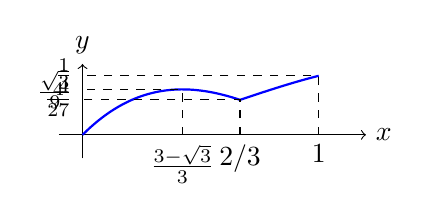
\begin{tikzpicture}[scale=3]
    \draw[->] (-0.1,0) -- (1.2,0) node[right] {$x$};
    \draw[->] (0,-0.1) -- (0,0.3) node[above] {$y$};
    
    % h(x) from 0 to 2/3
    \draw[domain=0:0.6667, smooth, variable=\x, blue, thick] plot ({\x}, {0.5*(2*\x - \x*\x)*(1-\x)});
    % g(x) from 2/3 to 1
    \draw[domain=0.6667:1, smooth, variable=\x, blue, thick] plot ({\x}, {0.25*(2-\x)*\x*\x});
    
    \draw[dashed] ({ (3-sqrt(3))/3 }, 0) node[below] {$\frac{3-\sqrt{3}}{3}$} -- ({ (3-sqrt(3))/3 }, {sqrt(3)/9}) -- (0, {sqrt(3)/9}) node[left] {$\frac{\sqrt{3}}{9}$};
    \draw[dashed] (0.6667, 0) node[below] {$2/3$} -- (0.6667, 4/27) -- (0, 4/27) node[left] {$\frac{4}{27}$};
    \draw[dashed] (1, 0) node[below] {$1$} -- (1, 0.25) -- (0, 0.25) node[left] {$\frac{1}{4}$};
\end{tikzpicture}
\end{center}

\end{document}
